\chapter{Zero knowledge proofs}\label{Zero-knowledge-proofs}

The notion of \emph{proof} is central to so many fields. In mathematics,
we want to prove that a certain assertion is correct. In other sciences,
we often want to accumulate a preponderance of evidence (or statistical
significance) to reject certain hypothesis. In criminal law the
prosecution famously needs to prove its case ``beyond a reasonable
doubt''. Cryptography turns out to give some new twists on this ancient
notion.

Typically a proof that some assertion X is true, also reveals some
information about \emph{why} X is true. When Hercule Poirot proves that
Norman Gale killed Madame Giselle he does so by showing \emph{how} Gale
committed the murder by dressing up as a flight attendant and stabbing
Madame Gisselle with a poisoned dart. Could Hercule convince us beyond a
reasonable doubt that Gale did the crime without giving any information
on \emph{how} the crime was committed? Can the Russians prove to the
U.S. that a sealed box contains an authentic nuclear warhead without
revealing anything about its design? Can I prove to you that the number
\(m=385,608,108,395,369,363,400,501,273,594,475,104,405,448,848,047,062,278,473,983\)
has a prime factor whose last digit is \(7\) without giving you any
information about \(m\)'s prime factors? We won't answer the first
question, but will show some insights on the latter two.\footnote{In
  case you are curious, the factors of \(m\) are
  \(1,172,192,558,529,627,184,841,954,822,099\) and
  \(328,963,108,995,562,790,517,498,071,717\).}

\emph{Zero knowledge proofs} are proofs that fully convince that a
statement is true without yielding \emph{any additional knowledge}. So,
after seeing a zero knowledge proof that \(m\) has a factor ending with
\(7\), you'll be no closer to knowing \(m\)'s factorization than you
were before. Zero knowledge proofs were invented by Goldwasser, Micali
and Rackoff in 1982 and have since been used in great many settings. How
would you achieve such a thing, or even define it? And why on earth
would it be useful? This is the topic of this lecture.

\section{Applications for zero knowledge
proofs.}\label{Applications-for-zero-knowledg}

Before we talk about how to achieve zero knowledge, let us discuss some
of its potential applications:

\subsection{Nuclear disarmament}\label{Nuclear-disarmament}

The United States and Russia have reached a dangerous and expensive
equilibrium by which each has about
\href{https://www.armscontrol.org/factsheets/Nuclearweaponswhohaswhat}{7000
nuclear warheads}, much more than is needed to decimate each others'
population (and the population of much of the rest of the
world).\footnote{To be fair, ``only'' about 170 million Americans live
  in the
  \href{https://www.currentresults.com/Weather-Extremes/US/largest-cities-list.php}{50
  largest metropolitan areas} and so arguably many people will survive
  at least the initial impact of a nuclear war, though it had been
  estimated that even a ``small'' nuclear war involving detonation of
  100 not too large warheads could have
  \href{http://onlinelibrary.wiley.com/doi/10.1002/2013EF000205/full}{devastating
  global consequences}.} Having so many weapons increases the chance of
``leakage'' of weapons, or of an accidental launch (which can result in
an all out war) through fault in communications or rogue commanders.
This also threatens the delicate balance of the
\href{https://en.wikipedia.org/wiki/Treaty_on_the_Non-Proliferation_of_Nuclear_Weapons}{Non-Proliferation
Treaty} which at its core is a bargain where non-weapons states agree
not to pursue nuclear weapons and the five nuclear weapon states agree
to make progress on nuclear disarmament. These huge quantities of
nuclear weapons are not only dangerous, as they increase the chance of a
leak or of an individual failure or rogue commander causing a world
catastrophe, but also extremely expensive to maintain.

For all of these reasons, in 2009, U.S. President Obama called to set as
a long term goal a ``world without nuclear weapons'' and in 2012 talked
about concretely talking to Russia about reducing ``not only
our~strategic nuclear warheads, but also tactical weapons and warheads
in reserve''. On the other side, Russian President Putin has said
already in 2000 that he sees ``no obstacles that could hamper future
deep cuts of strategic offensive armaments''. (Though as of 2018,
political winds on both sides have shifted away from disarmament and
more toward armament.)

There are many reasons why progress on nuclear disarmament has been so
slow, and most of them have nothing to do with zero knowledge or any
other piece of technology. But there are some technical hurdles as well.
One of those hurdles is that for the U.S. and Russia to go beyond
restricting the number of \emph{deployed} weapons to significantly
reducing the \emph{stockpiles}, they need to find a way for one country
to verifiably prove that it has dismantled warheads. As mentioned in my
\href{http://www.nature.com/nature/journal/v510/n7506/full/nature13457.html}{work
with Glaser and Goldston} (see also
\href{http://nuclearfutures.princeton.edu/warhead-verification/}{this
page}), a key stumbling block is that the design of a nuclear warhard is
of course highly classified and about the last thing in the world that
the U.S. would like to share with Russia and vice versa. So, how can the
U.S. convince the Russian that it has destroyed a warhead, when it
cannot let Russian experts anywhere near it?

\subsection{Voting}\label{Voting}

Electronic voting has been of great interest for many reasons. One
potential advantage is that it could allow completely transparent vote
counting, where every citizen could verify that the votes were counted
correctly. For example, Chaum suggested an approach to do so by
publishing an encryption of every vote and then having the central
authority \emph{prove} that the final outcome corresponds to the counts
of all the plaintexts. But of course to maintain voter privacy, we need
to prove this without actually revealing those plaintexts. Can we do so?

\subsection{More applications}\label{More-applications}

I chose these two examples above precisely because they are hardly the
first that come to mind when thinking about zero knowledge. Zero
knowledge has been used for many cryptographic applications. One such
application (originating from work of Fiat and Shamir) is the use for
\emph{identification protocols}. Here Alice knows a solution \(x\) to a
puzzle \(P\), and proves her identity to Bob by, for example, providing
an encryption \(c\) of \(x\) and proving in zero knowledge that \(c\) is
indeed an encryption of a solution for \(P\).\footnote{As we'll see,
  technically what Alice needs to do in such a scenario is use a
  \emph{zero knowledge proof of knowledge} of a solution for \(P\).} Bob
can verify the proof, but because it is zero knowledge, learns nothing
about the solution of the puzzle and will not be able to impersonate
Alice. An alternative approach to such identification protocols is
through using \emph{digital signatures}; this connection goes both ways
and zero knowledge proofs have been used by Schnorr and others as a
basis for signature schemes.

Another very generic application is for ``compiling protocols''. As
we've seen time and again, it is often much easier to handle
\emph{passive} adversaries than \emph{active} ones. (For example, it's
much easier to get CPA security against the eavesdropping Eve than CCA
security against the person-in-the-middle Mallory.) Thus it would be
wonderful if we could ``compile'' a protocol that is secure with respect
to passive attacks into one that is secure with respect to active ones.
As was first shown by Goldreich, Micali, and Wigderson, zero knowledge
proofs yield a very general such compiler. The idea is that all parties
prove in zero knowledge that they follow the protocol's specifications.
Normally, such proofs might require the parties to reveal their secret
inputs, hence violating security, but zero knowledge precisely
guarantees that we can verify correct behaviour without access to these
inputs.

\section{Defining and constructing zero knowledge
proofs}\label{Defining-and-constructing-zero}

So, zero knowledge proofs are wonderful objects, but how do we get them?
In fact, we haven't answered the even more basic question of how do we
\emph{define} zero knowledge? We have to start by the most basic task of
defining what we mean by a \emph{proof}.

A \emph{proof system} can be thought of as an algorithm \(V\) (for
``verifier'') that takes as input a \emph{statement} which is some
string \(x\) and another string \(\pi\) known as the \emph{proof} and
outputs \(1\) if and only if \(\pi\) is a valid proof that the statement
\(x\) is correct. For example:

\begin{itemize}
\item
  In \emph{Euclidean geometry}, \emph{statements} are geometric facts
  such as ``in any triangle the degrees sum to 180 degrees'' and the
  \emph{proofs} are step by step derivations of the statements from the
  five basic
  \href{https://en.wikipedia.org/wiki/Euclidean_geometry}{postulates}.
\item
  In
  \href{https://en.wikipedia.org/wiki/Zermelo\%E2\%80\%93Fraenkel_set_theory}{\emph{Zermelo-Fraenkel
  + Axiom of Choice (ZFC)}} a \emph{statement} is some purported fact
  about sets (e.g., the Riemann Hypothesis\footnote{Integers can be
    coded as sets in various ways. For example, one can encode \(0\) as
    \(\emptyset\) and if \(N\) is the set encoding \(n\), we can encode
    \(n+1\) using the \(n+1\)-element set \(\{ N \} \cup N\).}), and a
  \emph{proof} is a step by step derivation of it from the axioms.
\item
  We can many define other ``theories''. For example, a theory where the
  statements are pairs \((x,m)\) such that \(x\) is a quadratic residue
  modulo \(m\) and a proof for \(x\) is the number \(s\) such that
  \(x=s^2 \pmod{m}\), or a theory where the theorems are
  \emph{Hamiltonian} graphs \(G\) (graphs on \(n\) vertices that contain
  an \(n\)-long cycle) and the proofs are the description of the cycle.
\end{itemize}

All these proof systems have the property that the verifying algorithm
\(V\) is \emph{efficient}. Indeed, that's the whole point of a proof
\(\pi\)- it's a sequence of symbols that makes it easy to verify that
the statement is true.

To achieve the notion of zero knowledge proofs, Goldwasser and Micali
had to consider a generalization of proofs from static sequences of
symbols to \emph{interactive probabilistic protocols} between a prover
and a verifier. Let's start with an informal example. The vast majority
of humans have three types of cone cells in their eyes. This is the
reason why
\href{http://www.patarnott.com/atms749/pdf/blueSkyHumanResponse.pdf}{we
perceive the sky as blue} (see also
\href{https://www.forbes.com/sites/briankoberlein/2017/01/11/earths-skies-are-violet-we-just-see-them-as-blue/\#33aaaf0f735f}{this}),
despite its color being quite a different spectrum than the blue of the
rainbow, is that the projection of the sky's color to our cones is
closest to the projection of blue. It has been suggested that a tiny
fraction of the human population might have four functioning cones (in
fact, only women, as it would require two X chromosomes and a certain
mutation). How would a person \emph{prove} to another that she is a in
fact such a
\href{https://en.wikipedia.org/wiki/Tetrachromacy}{tetrachromat} ?

\begin{quote}
\textbf{Proof of tetrachromacy:}

Suppose that Alice is a tetrachromat and can distinguish between the
colors of two pieces of plastic that would be identical to a trichromat.
She wants to prove to a trichromat Bob that the two pieces are not
identical. She can do this as follows:

Alice and Bob will repeat the following experiment \(n\) times: Alice
turns her back and Bob tosses a coin and with probability 1/2 leaves the
pieces as they are, and with probability 1/2 switches the right piece
with the left piece. Alice needs to guess whether Bob switched the
pieces or not.

If Alice is successful in all of the \(n\) repetitions then Bob will
have \(1-2^{-n}\) confidence that the pieces are truly different.
\end{quote}

We now consider a more ``mathematical'' example along similar lines.
Recall that if \(x\) and \(m\) are numbers then we say that \(x\) is a
\emph{quadratic residue} modulo \(m\) if there is some \(s\) such that
\(x=s^2 \pmod{m}\). Let us define the function
\(\ensuremath{\mathit{NQR}}(m,x)\) to output \(1\) if and only if
\(x \neq s^2 \pmod{m}\) for every \(s \in \{0,\ldots, m-1\}\). There is
a very simple way to prove statements of the form
``\(\ensuremath{\mathit{NQR}}(m,x)=0\)'': just give out \(s\). However,
here is an interactive proof system to prove statements of the form
``\(\ensuremath{\mathit{NQR}}(m,x)=1\)'':

\begin{itemize}
\item
  We have two parties: \textbf{Alice} and \textbf{Bob}. The
  \textbf{common input} is \((m,x)\) and Alice wants to convince Bob
  that \(\ensuremath{\mathit{NQR}}(m,x)=1\). (That is, that \(x\) is
  \emph{not} a quadratic residue modulo \(m\)).
\item
  We assume that Alice can compute \(\ensuremath{\mathit{NQR}}(m,w)\)
  for every \(w\in \{0,\ldots,m-1\}\) but Bob is polynomial time.
\item
  The protocol will work as follows:
\end{itemize}

\begin{enumerate}
\def\labelenumi{\arabic{enumi}.}
\item
  Bob will pick some random \(s\in \Z^*_m\) (e.g., by picking a random
  number in \(\{1,\ldots,m-1\}\) and discard it if it has nontrivial
  g.c.d. with \(m\)) and toss a coin \(b\in\{0,1\}\). If \(b=0\) then
  Bob will send \(s^2 \pmod{m}\) to Alice and otherwise he will send
  \(xs^2 \pmod{m}\) to Alice.
\item
  Alice will use her ability to compute
  \(\ensuremath{\mathit{NQR}}(m,\cdot)\) to respond with \(b'=0\) if Bob
  sent a quadratic residue and with \(b'=1\) otherwise.
\item
  Bob \emph{accepts} the proof if \(b=b'\).
\end{enumerate}

To see that Bob will indeed accept the proof, note that if \(x\) is a
non-residue then \(xs^2\) will have to be a non-residue as well (since
if it had a root \(s'\) then \(s's^{-1}\) would be a root of \(x\)).
Hence it will always be the case that \(b'=b\).

Moreover, if \(x\) \emph{was} a quadratic residue of the form
\(x=s'^2 \pmod{m}\) for some \(s'\), then \(xs^2=(s's)^2\) is simply a
random quadratic residue, which means that in this case Bob's message is
distributed the same regardless of whether \(b=0\) or \(b=1\), and no
matter what she does, Alice has probability at most \(1/2\) of guessing
\(b\). Hence if Alice is always successful than after \(n\) repetitions
Bob would have \(1-2^{-n}\) confidence that \(x\) is indeed a
non-residue modulo \(m\).

\begin{pause} \label[pause]{Please-stop-and-make-sure-you-}

Please stop and make sure you see the similarities between this protocol
and the one for demonstrating that the two pieces of plastic do not have
identical colors.

\end{pause}

Let us now make the formal definition:

\hypertarget{proofsystemdef}{}
\begin{definition}[Proof systems] \label[definition]{proofsystemdef}

Let \(f:\{0,1\}^* \rightarrow \{0,1\}\) be some function. A
\emph{probabilistic proof for \(f\)} (i.e., a proof for statements of
the form ``\(f(x)=1\)'') is a pair of interactive algorithms \((P,V)\)
such that \(V\) runs in polynomial time and they satisfy:

\begin{itemize}
\item
  \textbf{Completeness:} If \(f(x)=1\) then on input \(x\), if \(P\) and
  \(V\) are given input \(x\) and interact, then at the end of the
  interaction \(V\) will output \texttt{Accept} with probability at
  least \(0.9\).
\item
  \textbf{Soundness:} If If \(f(x)=0\) then for any arbitrary (efficient
  or non efficient) algorithm \(P^*\), if \(P^*\) and \(V\) are given
  input \(x\) and interact then at the end \(V\) will output
  \texttt{Accept} with probability at most \(0.1\)
\end{itemize}

\end{definition}

\hypertarget{funclangrem}{}
\begin{remark}[Functions vs languages] \label[remark]{funclangrem}

In many texts proof systems are defined with respect to \emph{languages}
as opposed to \emph{functions}. That is, instead of talking about a
function \(f:\{0,1\}^* \rightarrow \{0,1\}\) we talk about a
\emph{lanugage} \(L \subseteq \{0,1\}^*\). These two viewpoints are
completely equivalent via the mapping \(f \longleftrightarrow L\) where
\(L = \{ x \;| f(x) = 1 \}\).

\end{remark}

Note that we don't necessarily require the prover to be efficient (and
indeed, in some cases it might not be). On the other hand, our soundness
condition holds even if the prover uses a non efficient
strategy.\footnote{People have considered the notion of zero knowledge
  systems where soundness holds only with respect to efficient provers;
  these are known as \emph{argument systems}.} We say that a proof
system has an \emph{efficient prover} if there is an NP-type proof
system \(\Pi\) for \(L\) (that is some efficient algorithm \(\Pi\) such
that there exists \(\pi\) with \(\Pi(x,\pi)=1\) iff \(x\in L\) and such
that \(\Pi(x,\pi)=1\) implies that \(|\pi|\leq poly(|x|)\)), such that
the strategy for \(P\) can be implemented efficiently given any static
proof \(\pi\) for \(x\) in this system.

\hypertarget{strategies}{}
\begin{remark}[Notation for strategies] \label[remark]{strategies}

Up until now, we always considered cryptographic protocols where Alice
and Bob trusted one another, but were worried about some adversary
controlling the channel between them. Now we are in a somewhat more
``suspicious'' setting where the parties do not fully trust one another.
In such protocols there is always a ``prescribed'' or \textbf{honest}
strategy that a particular party \emph{should} follow, but we generally
don't want the other parties' security to rely on someone else's good
intention, and hence analyze also the case where a party uses an
arbitrary \textbf{malicious} strategy. We sometimes also consider the
\textbf{honest but curious} case where the adversary is passive and only
collects information, but does not deviate from the prescribed strategy.

Protocols typically only guarantee security for party A when it behaves
honestly - a party can always chose to violate its own security and
there is not much we can (or should?) do about it.

\end{remark}

\section{Defining zero knowledge}\label{Defining-zero-knowledge}

So far we merely defined the notion of an interactive proof system, but
we need to define what it means for a proof to be \emph{zero knowledge}.
Before we attempt a definition, let us consider an example. Going back
to the notion of quadratic residuosity, suppose that \(x\) and \(m\) are
public and Alice knows \(s\) such that \(x=s^2 \pmod{m}\). She wants to
convince Bob that this is the case. However she prefers not to reveal
\(s\). Can she convince Bob that such an \(s\) exist without revealing
any information about it? Here is a way to do so:

\paragraph{Protocol ZK-QR:} Public input for Alice and Bob: \(x,m\);
Alice's private input is \(s\) such that \(x=s^2 \pmod{m}\).

\begin{enumerate}
\def\labelenumi{\arabic{enumi}.}
\item
  Alice will pick a random \(s'\) and send to Bob
  \(x' = xs'^2 \pmod{m}\).
\item
  Bob will pick a random bit \(b\in\{0,1\}\) and send \(b\) to Alice.
\item
  If \(b=0\) then Alice reveals \(ss'\), hence giving out a root for
  \(x'\); if \(b=1\) then Alice reveals \(s'\), hence showing a root for
  \(x'x^{-1}\).
\item
  Bob checks that the value \(s''\) revealed by Alice is indeed a root
  of \(x'x^{-b}\), if so then it ``accepts'' the proof.
\end{enumerate}

If \(x\) was \emph{not} a quadratic residue then no matter how \(x'\)
was chosen, either \(x'\) or \(x'x^{-1}\) is \emph{not} a residue and
hence Bob will reject the proof with probability at least \(1/2\). By
repeating this \(n\) times, we can reduce the probability of Bob
accepting a the proof of a non residue to \(2^{-n}\).

On the other hand, we claim that we didn't really reveal anything about
\(s\). Indeed, if Bob chooses \(b=0\), then the two messages
\((x',ss')\) he sees can be thought of as a random quadratic residue
\(x'\) and its root. If Bob chooses \(b=1\) then after dividing by \(x\)
(which he could have done by himself) he still gets a random residue
\(x''\) and its root \(s'\). In both cases, the distribution of these
two messages is completely independent of \(s\), and hence intuitively
yields no additional information about it beyond whatever Bob knew
before.

To define zero knowledge mathematically we follow the following
intuition:

\begin{quote}
\emph{A proof system is zero knowledge if the verifier did not learn
anything after the interaction that he could not have learned on his
own.}
\end{quote}

Here is how we formally define this:

\hypertarget{zkpdef}{}
\begin{definition}[Zero knowledge proofs] \label[definition]{zkpdef}

A proof system \((P,V)\) for \(f\) is \emph{zero knowledge} if for every
efficient verifier strategy \(V^*\) there exists an efficient
probabilistic algorithm \(S^*\) (known as the \emph{simulator}) such
that for every \(x\) s.t. \(f(x)=1\), the following random variables are
computationally indistinguishable:

\begin{itemize}
\item
  The output of \(V^*\) after interacting with \(P\) on input \(x\).
\item
  The output of \(S^*\) on input \(x\).
\end{itemize}

\end{definition}

That is, we can show the verifier does not gain anything from the
interaction, because no matter what algorithm \(V^*\) he uses, whatever
he learned as a result of interacting with the prover, he could have
just as equally learned by simply running the standalone algorithm
\(S^*\) on the same input.

\hypertarget{simulationrem}{}
\begin{remark}[The simulation paradigm] \label[remark]{simulationrem}

The natural way to define security is to say that a system is secure if
some ``laundry list'' of bad outcomes X,Y,Z can't happen. The definition
of zero knowledge is different. Rather than giving a list of the events
that are \emph{not allowed} to occur, it gives a maximalist
\emph{simulation} condition.

At its heart the definition of zero knowledge says the following:
clearly, we cannot prevent the verifier from running an efficient
algorithm \(S^*\) on the public input, but we want to ensure that this
is the most he can learn from the interaction. This \emph{simulation
paradigm} has become the standard way to define security of a great many
cryptographic applications. That is, we bound what an adversary Eve can
learn by postulating some hypothetical adversary Lilith that is under
much harsher conditions (e.g., does not get to interact with the prover)
and ensuring that Eve cannot learn anything that Lilith couldn't have
learned either. This has an advantage of being the most conservative
definition possible, and also phrasing security in \emph{positive}
terms- there exists a simulation - as opposed to the typical
\emph{negative} terms - events X,Y,Z can't happen. Since it's often
easier for us to think of positive terms, paradoxically sometimes this
stronger security condition is easier to prove. Zero knowledge is in
some sense the simplest setting of the simulation paradigm and we'll see
it time and again in dealing with more advanced notions.

\end{remark}

The definition of zero knowledge is confusing since intuitively one
thing that if the verifier gained confidence that the statement is true
than surely he must have learned \emph{something}. This is another one
of those cases where cryptography is counterintuitive. To understand it
better, it is worthwhile to see the formal proof that the protocol above
for quadratic residousity is zero knowledge:

\hypertarget{zkqrthm}{}
\begin{theorem}[Zero knowledge for quadratic residuosity] \label[theorem]{zkqrthm}

Protocol ZK-QR above is a zero knowledge protocol.

\end{theorem}

\begin{proof} \label[proof]{Let-V-be-an-arbitrary-efficien}

Let \(V^*\) be an arbitrary efficient strategy for Bob. Since Bob only
sends a single bit, we can think of this strategy as composed of two
functions:

\begin{itemize}
\item
  \(V_1(x,m,x')\) outputs the bit \(b\) that Bob chooses on input
  \(x,m\) and after Alice's first message is \(x'\).
\item
  \(V_2(x,m,x',s'')\) is whatever Bob outputs after seeing Alice's
  response \(s''\) to the bit \(b\).
\end{itemize}

Both \(V_1\) and \(V_2\) are efficiently computable. We now need to come
up with an efficient simulator \(S^*\) that is a standalone algorithm
that on input \(x,m\) will output a distribution indistinguishable from
the output \(V^*\). The simulator \(S^*\) will work as follows:

\begin{enumerate}
\def\labelenumi{\arabic{enumi}.}
\item
  Pick \(b'\leftarrow_R\{0,1\}\).
\item
  Pick \(s''\) at random in \(\Z^*_m\). If \(b=0\) then let
  \(x'={s''}^2 \pmod{m}\). Otherwise output \(x'=x{s''}^2 \pmod{m}\).
\item
  Let \(b=V_1(x,m,x')\). If \(b \neq b'\) then go back to step 1.
\item
  Output \(V_2(x,m,x',s'')\).
\end{enumerate}

The correctness of the simulator follows from the following claims (all
of which assume that \(x\) is actually a quadratic residue, since
otherwise we don't need to make any guarantees and in any case Alice's
behaviour is not well defined):

\textbf{Claim 1:} The distribution of \(x'\) computed by \(S^*\) is
identical to the distribution of \(x'\) chosen by Alice.

\textbf{Claim 2:} With probability at least \(1/2\), \(b'=b\).

\textbf{Claim 3:} Conditioned on \(b=b'\) and the value \(x'\) computed
in step 2, the value \(s''\) computed by \(S^*\) is identical to the
value that Alice sends when her first message is \(X'\) and Bob's
response is \(b\).

Together these three claims imply that in expectation \(S^*\) only
invokes \(V_1\) and \(V_2\) a constant number of times (since every time
it goes back to step 1 with probability at most \(1/2\)). They also
imply that the output of \(S^*\) is in fact identical to the output of
\(V^*\) in a true interaction with Alice. Thus, we only need to prove
the claims, which is actually quite easy:

\textbf{Proof of Claim 1:} In both cases, \(x'\) is a random quadratic
residue. QED

\textbf{Proof of Claim 2:} This is a corollary of Claim 1; since the
distribution of \(x'\) is identical to the distribution chosen by Alice,
in particular \(x'\) gives out no information about the choice of
\(b'\). QED

\textbf{Proof of Claim 3:} This follows from a direct calculation. The
value \(s''\) sent by Alice is a square root of \(x'\) if \(b=0\) and of
\(x'x^{-1}\) if \(x=1\). But this is identical to what happens for
\(S^*\) if \(b=b'\). QED

Together these complete the proof of the theorem.

\end{proof}

\cref{zkqrthm} is interesting but not yet good enough to guarantee
security in practice. After all, the protocol that we really need to
show is zero knowledge is the one where we repeat this procedure \(n\)
times. This is a general theorem that if a protocol is zero knowledge
then repeating it polynomially many times one after the other (so called
``sequential repetition'') preserves zero knowledge. You can think of
this as cryptography's version of the equality ``\(0+0=0\)'', but as
usual, intuitive things are not always correct and so this theorem does
require (a not super trivial) proof. It is a good exercise to try to
prove it on your own. There are known ways to achieve zero knowledge
with negligible soundness error and a \emph{constant} number of
communication rounds, see Goldreich's book (Vol 1, Sec 4.9).

\section{Zero knowledge proof for
Hamiltonicity.}\label{Zero-knowledge-proof-for-Hamil}

We now show a proof for another language. Suppose that Alice and Bob
know an \(n\)-vertex graph \(G\) and Alice knows a \emph{Hamiltonian
cycle} \(C\) in this graph (i.e.. a length \(n\) simple cycle- one that
traverses all vertices exactly once). Here is how Alice can prove that
such a cycle exists without revealing any information about it:

\paragraph{Protocol ZK-Ham:}

\begin{enumerate}
\def\labelenumi{\arabic{enumi}.}
\setcounter{enumi}{-1}
\item
  \textbf{Common input:} graph \(H\) (in the form of an \(n\times n\)
  adjacency matrix); \textbf{Alice's private input:} a Hamiltonian cycle
  \(C=(C_1,\ldots,C_n)\) which are distinct vertices such that
  \((C_\ell,C_{\ell+1})\) is an edge in \(H\) for all
  \(\ell\in\{1,\ldots,n-1\}\) and \((C_n,C_1)\) is an edge as well.
\item
  Bob chooses a random string \(z\in \{0,1\}^{3n}\)
\item
  Alice chooses a random permutation \(\pi\) on \(\{1,\ldots, n\}\) and
  let \(M\) be the \(\pi\)-permuted adjacency matrix of \(H\) (i.e.,
  \(M_{\pi(i),\pi(j)}=1\) iff \((i,j)\) is an edge in \(H\)). For every
  \(i,j\), Alice chooses a random string \(x_{i,j} \in \{0,1\}^n\) and
  let \(y_{i,j}=G(x_{i,j})\oplus M_{i,j}z\), where
  \(G:\{0,1\}^n\rightarrow\{0,1\}^{3n}\) is a pseudorandom generator.
  She sends \(\{ y_{i,j} \}_{i,j \in [n]}\) to Bob.
\item
  Bob chooses a bit \(b\in\{0,1\}\).
\item
  If \(b=0\) then Alice sends out \(\pi\) and the strings
  \(\{ x_{i,j} \}\) for all \(i,j\); If \(b=1\) then Alice sends out the
  \(n\) strings
  \(x_{\pi(C_1),\pi(C_2)}\),\(\ldots\),\(x_{\pi(C_n),\pi(C_1)}\)
  together with their indices.
\item
  If \(b=0\) then Bob computes \(M\) to be the \(\pi\)-permuted
  adjacency matrix of \(H\) and verifies that all the \(y_{i,j}\)'s were
  computed from the \(x_{i,j}\)'s appropriately. If \(b=1\) then verify
  that the indices of the strings \(\{ x_{i,j } \}\) sent by Alice form
  a cycle and that indeed \(y_{i,j}=G(x_{i,j})\oplus z\) for every
  string \(x_{i,j}\) that was sent by Alice.
\end{enumerate}

\hypertarget{zkhamthm}{}
\begin{theorem}[Zero Knowledge proof for Hamiltonian Cycle] \label[theorem]{zkhamthm}

Protocol ZK-Ham is a zero knowledge proof system for the language of
Hamiltonian graphs.\footnote{Goldreich, Micali and Wigderson were the
  first to come up with a zero knowledge proof for an NP complete
  problem, though the Hamiltoncity protocol here is from a later work by
  Blum. We use Naor's commitment scheme.}

\end{theorem}

\begin{proof} \label[proof]{We-need-to-prove-completeness-}

We need to prove \textbf{completeness}, \textbf{soundness}, and
\textbf{zero knowledge}.

\textbf{Completeness} can be easily verified, and so we leave this to
the reader.

For \textbf{soundness}, we recall that (as we've seen before) with
extremely high probability the sets \(S_0=\{ G(x) : x\in\{0,1\}^n \}\)
and \(S_1 = \{ G(x)\oplus z : x\in\{0,1\}^n \}\) will be disjoint (this
probability is over the choice of \(z\) that is done by the verifier).
Now, assuming this is the case, given the messages \(\{ y_{i,j} \}\)
sent by the prover in the first step, define an \(n\times n\) matrix
\(M'\) with entries in \(\{0,1,?\}\) as follows: \(M'_{i,j}=0\) if
\(y_{i,j}\in S_0\) , \(M'_{i,j}=1\) if \(y_{i,j}\in S_1\) and
\(M'_{i,j}=?\) otherwise.

We split into two cases. The first case is that there exists some
permutation \(\pi\) such that \textbf{(i)} \(M'\) is a \(\pi\)-permuted
version of the input graph \(G\) and \textbf{(ii)} \(M'\) contains a
Hamiltonian cycle. Clearly in this case \(G\) contains a Hamiltonian
cycle as well, and hence we don't need to consider it when analyzing
soundness. In the other case we claim that with probability at least
\(1/2\) the verifier will reject the proof. Indeed, if \textbf{(i)} is
violated then the proof will be rejected if Bob chooses \(b=0\) and if
\textbf{(ii)} is violated then the proof will be rejected if Bob chooses
\(b=1\).

We now turn to showing \textbf{zero knowledge}. For this we need to
build a \emph{simulator} \(S^*\) for an arbitrary efficient strategy
\(V^*\) of Bob. Recall that \(S^*\) gets as input the graph \(H\) (but
not the \emph{Hamiltonian} cycle \(C\)) and needs to produce an output
that is indistinguishable from the output of \(V^*\). It will do so as
follows:

\begin{enumerate}
\def\labelenumi{\arabic{enumi}.}
\setcounter{enumi}{-1}
\item
  Pick \(b'\in\{0,1\}\).
\item
  Let \(z\in \{0,1\}^{3n}\) be the first message computed by \(V^*\) on
  input \(H\).
\item
  If \(b'=0\) then \(S^*\) computes the second message as Alice does:
  chooses a random permutation \(\pi\) on \(\{1,\ldots, n\}\) and let
  \(M\) be the \(\pi\)-permuted adjacency matrix of \(H\) (i.e.,
  \(M_{\pi(i),\pi(j)}=1\) iff \((i,j)\) is an edge in \(H\)). In
  contrast, if \(b'=1\) then \(S^*\) lets \(M\) be the all \(1'\)
  matrix. For every \(i,j\), \(S^*\) chooses a random string
  \(x_{i,j} \in \{0,1\}^n\) and let
  \(y_{i,j}=G(x_{i,j})\oplus M_{i,j}z\), where
  \(G:\{0,1\}^n\rightarrow\{0,1\}^{3n}\) is a pseudorandom generator.
\item
  Let \(b\) be the output of \(V^*\) when given the input \(H\) and the
  first message \(\{ y_{i,j} \}\) computed as above. If \(b\neq b'\)
  then go back to step 0.
\item
  We compute the fourth message of the protocol similarly to how Alice
  does it: if \(b=0\) then it consists of \(\pi\) and the strings
  \(\{ x_{i,j} \}\) for all \(i,j\); If \(b=1\) then we pick a random
  length-\(n\) cycle \(C'\) and the message consists of the \(n\)
  strings \(x_{C'_1,C'_2}\),\(\ldots\),\(x_{C'_n,C'_1}\) together with
  their indices.
\item
  Output whatever \(V^*\) outputs when given the prior message.
\end{enumerate}

We prove the output of the simulator is indistinguishable from the
output of \(V^*\) in an actual interaction by the following claims:

\textbf{Claim 1:} The message \(\{ y_{i,j} \}\) computed by \(S^*\) is
computationally indistinguishable from the first message computed by
Alice.

\textbf{Claim 2:} The probability that \(b=b'\) is at least \(1/3\).

\textbf{Claim 3:} The fourth message computed by \(S^*\) is
computationally indistinguishable from the fourth message computed by
Alice.

We will simply sketch here the proofs (again see Goldreich's book for
full proofs):

For Claim 1, note that if \(b'=0\) then the message is \emph{identical}
to the way Alice computes it. If \(b'=1\) then the difference is that
\(S^*\) computes some strings \(y_{i,j}\) of the form \(G(x_{i,j})+z\)
where Alice would compute the corresponding strings as \(G(x_{i,j})\)
this is indistinguishable because \(G\) is a pseudorandom generator (and
the distribution \(U_{3n}\oplus z\) is the same as \(U_{3n}\)).

Claim 2 is a corollary of Claim 1. If \(V^*\) managed to pick a message
\(b\) such that \(\Pr[ b=b' ] < 1/2 - negl(n)\) then in particular it
could distinguish between the first message of Alice (that is computed
independently of \(b'\) and hence contains no information about it) from
the first message of \(V^*\).

For Claim 3, note that again if \(b=0\) then the message is computed in
a way identical to what Alice does. If \(b=1\) then this message is also
computed in a way identical to Alice, since it does not matter if
instead of picking \(C'\) at random, we picked a random permutation
\(\pi\) and let \(C'\) be the image of the Hamiltonian cycle under this
permutation.

This completes the proof of the theorem.

\end{proof}

\subsection{Why is this interesting?}\label{Why-is-this-interesting}

The reason that a protocol for Hamiltonicity is more interesting than a
protocol for quadratic residuosity is that Hamiltonicity is an
NP-complete question. This means that for every other NP language \(L\),
we can use the reduction from \(L\) to Hamiltonicity combined with
protocol ZK-Ham to give a zero knowledge proof system for \(L\). In
particular this means that we can have zero knowledge proofs for the
following languages:

\begin{itemize}
\item
  The language of numbers \(m\) such that there exists a prime \(p\)
  dividing \(m\) whose remainder modulo \(10\) is \(7\).
\item
  The language of tuples \(X,e,c_1,\ldots,c_n\) such that \(c_i\) is an
  encryption of a number \(x_i\) with \(\sum x_i = X\). (This is
  essentially what we needed in the voting example above).
\item
  For every efficient function \(F\), the language of pairs \(x,y\) such
  that there exists some input \(r\) satisfying \(y=F(x\|r)\). (This is
  what we often need in the ``protocol compiling'' applications to show
  that a particular output was produced by the correct program \(F\) on
  public input \(x\) and private input \(r\).)
\end{itemize}


\begin{figure}
\centering
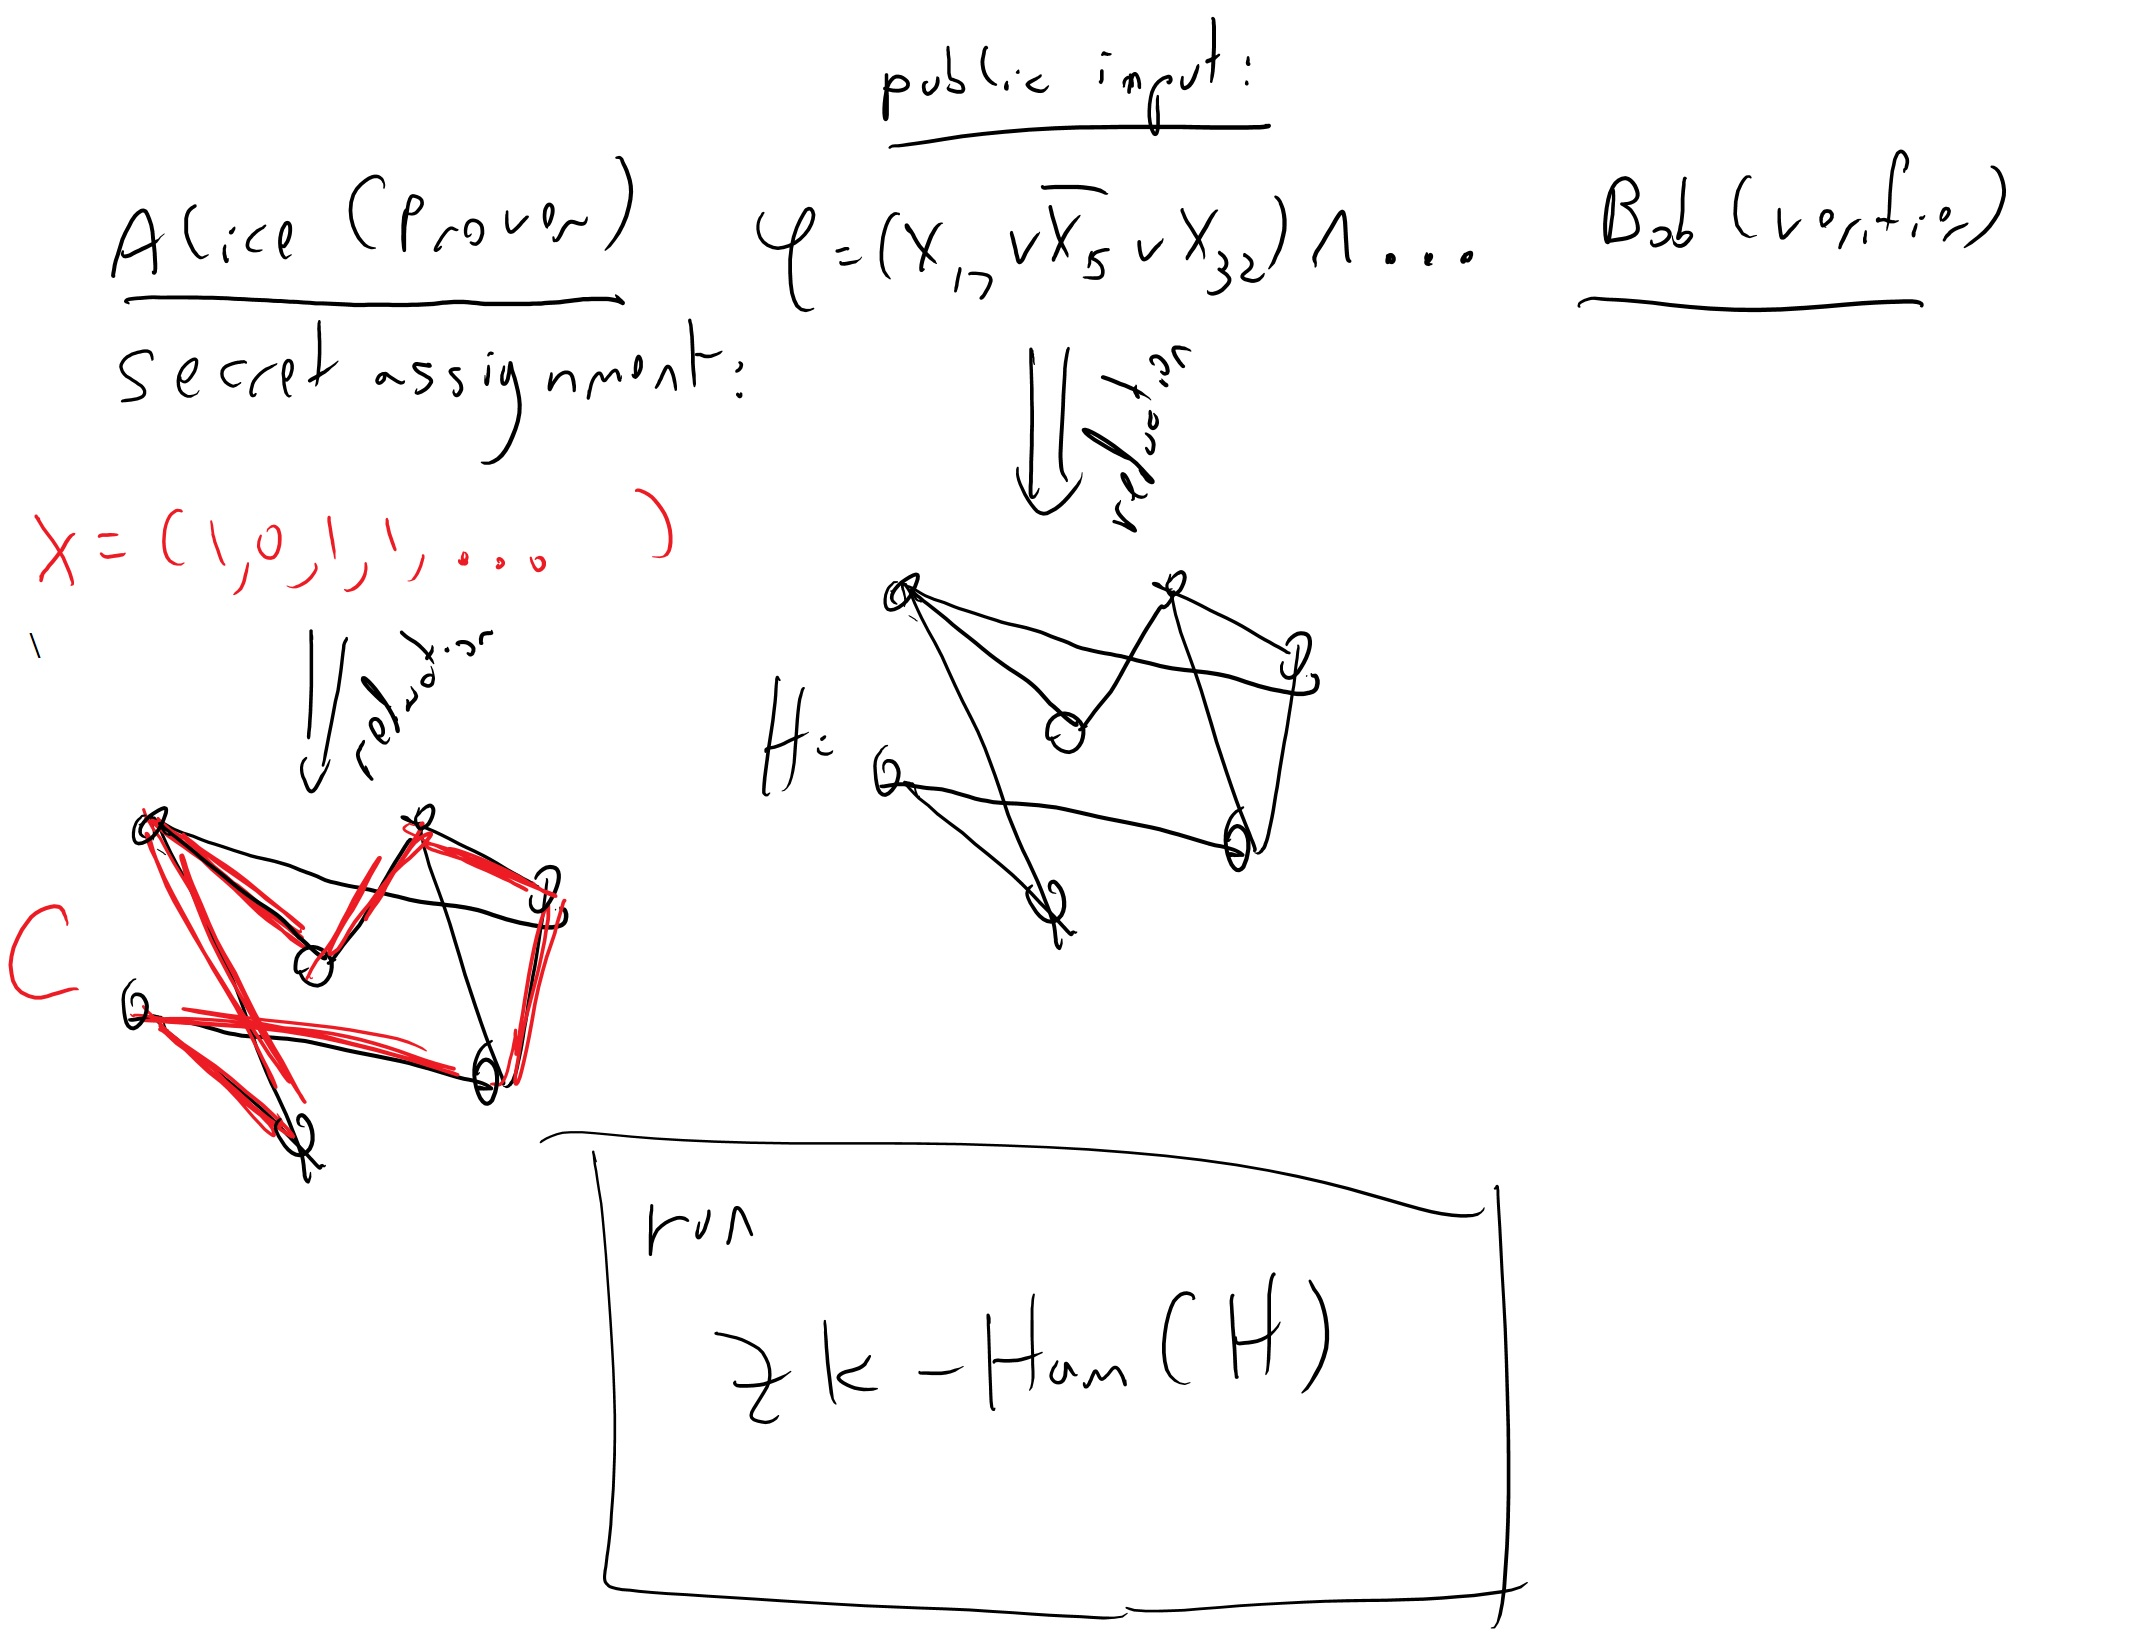
\includegraphics[width=\textwidth, height=0.25\paperheight, keepaspectratio]{../figure/zk-ham.jpg}
\caption{Using a zero knowledge protocol for Hamiltonicity we can obtain
a zero knowledge protocol for any language \(L\) in NP. For example, if
the public input is a SAT formula \(\varphi\) and the Prover's secret
input is a satisfying assignment \(x\) for \(\varphi\) then the verifier
can run the reduction on \(\varphi\) to obtain a graph \(H\) and the
prover can run the same reduction to obtain from \(x\) a Hamiltonian
cycle \(C\) in \(H\). They can then run the ZK-Ham protocol to prove
that indeed \(H\) is Hamiltonian (and hence the original formula was
satisfiable) without revealing any information the verifier could not
have obtain on his own.}
\label{tmplabelfig}
\end{figure}

\section{Parallel repetition and turning zero knowledge proofs to
signatures.}\label{Parallel-repetition-and-turnin}

While we talked about amplifying zero knowledge proofs by running them
\(n\) times one \emph{after} the other, one could also imagine running
the \(n\) copies \emph{in parallel}. It is not trivial that we get the
same benefit of reducing the error to \(2^{-n}\) but it turns out that
we do in the cases we are interested in here. Unfortunately, zero
knowledge is not necessarily preserved. It's an important open problem
whether zero knowledge is preserved for the ZK-Ham protocol mentioned
above.\\
However, Fiat and Shamir showed that in protocols (such as the ones we
showed here) where the verifier only sends random bits, then if we
replaced this verifier by a \emph{random function}, then both soundness
and zero knowledge are preserved. This suggests a \emph{non-interactive}
version of these protocols in the random oracle model, and this is
indeed widely used. Schnorr designed signatures based on this non
interactive version.

\subsection{``Bonus features'' of zero
knowledge}\label{Bonus-features-of-zero-knowled}

\begin{itemize}
\item
  Proof of knowledge
\item
  Deniability / non-transferability
\end{itemize}
